\documentclass[10pt,a4paper]{article}
\usepackage[utf8]{inputenc}
\usepackage[english]{babel}
\usepackage[T1]{fontenc}
\usepackage{amsmath}
\usepackage{amsfonts}
\usepackage{amssymb}
\usepackage{subcaption}
\usepackage{makeidx}
\usepackage{graphicx}
\usepackage{fourier}
\usepackage{listings}
\usepackage{color}
\usepackage{hyperref}
\usepackage[left=2cm,right=2cm,top=2cm,bottom=2cm]{geometry}
\author{Tommy Müller, Marcus Dittrich, Vincent Noculak}
\title{Zeeman-Effekt}

\lstset{language=C++,
	keywordstyle=\bfseries\color{blue},
	commentstyle=\itshape\color{red},
	stringstyle=\color{green},
	identifierstyle=\bfseries,
	frame=single}
\begin{document}

\maketitle
\newpage
\tableofcontents
\newpage

\section{Einleitung}

In dem Versuch, Mie-Streuung an levitierten Flüssigkeitströpfchen, soll die Streuung von Laserlicht an kleinen Glaskügelchen und Aerosoltröpfchen untersucht werden. Der Radius der Kügelchen ist in der Größenordnung der Lichtwellenlänge. Diese geladenen Teilchen werden in einer Paulfalle in schwebe gehalten. Das verdampfen der Aerosoltröpfchen kann ebenso beobachtet werden.

\section{Theorie}
\subsection{Paulfalle}

Wir betrachten ein Teilchen mit der Masse m und der Ladung q im Potenzial\\

$\Phi(\overrightarrow r) = V (\alpha x^2+\beta y^2+\gamma z^2)$\\


Am Anfang betrachten wir den Raum als ladungsfrei, daher gilt die Laplace - Gleichung.\\
\begin{equation}
\Delta \Phi = 0   \leftrightarrow \alpha + \beta + \gamma = 0
\label {1}
\end{equation}

Es gibt viele Lösungen für die Gleichung, eine mögliche Lösung ist:

$\alpha = \beta\ und\ \gamma = -2 \alpha$

Mit dieser Wahl erhalten wir das Potenzial

\begin{equation}
\Delta \Phi = \frac{V}{2r_0^2}(r^2-2z^2)
\label {2}
\end{equation}

Dieses Potenzial ist nach \ref {1} für konstantes Potenzial, es gibt keinen Ort mit minimalen Potenzials. Ändert man nun V in

V = V (t)= U-$V_0 \cos(\omega t)$

so ist damit die Konstruierung einer Teilchenfalle möglich. 
Die Bewegungsgleichung des Teilchens in z- und r- Richtung sind mit $\overrightarrow F = - Q \delta\overrightarrow \phi$ gegeben durch

\begin{equation}
\frac {d^2r}{dt^2} = \frac{Q}{r_0^2 m}(U-V_0 \cos(\omega t)r)
\label {3}
\end{equation}


\begin{equation}
\frac -{1}{2}\frac {d^2z}{dt^2} = \frac{Q}{r_0^2 m}(U-V_0 \cos(\omega t)z)
\label {4}
\end{equation}

Nach dem einsetzen erhalten wir zwei Differenzialgleiungen 


\begin{equation}
a_z = -2a_r =\frac{-8 Q U}{r_0^2 m \omega^2}\
,q_z = -2q_r =\frac{-4 Q V_0}{r_0^2 m \omega^2}; 2\epsilon = \omega t
\label {5}
\end{equation}

die Form der Mathieuschen Differenzialgleichung \\

$f``(\epsilon) + (a-2b \cos(2\epsilon))f(\epsilon) = 0$\\

Die Lösungen der Mathieuschen  Differenzialgleung sind bekannt. Diese ist in allgemeiner Form gegeben durch: \\\\


$f(\epsilon) = A e^{\mü \epsilon} \sum_{\infty}^\infty C_{2n} e^{i2n\epsilon}+B e^{-\mü \epsilon} \sum_{\infty}^\infty C_{2n} e^{-i2n\epsilon}$\\

Nun ist die Frage, ob die Teilchenbahn stabil ist, d.h. ot r(t) und z(t) in einem gewissen Abstand nicht überstreiten, für dies muss Re($\mü$) = 0 gelten. 
Die Größen für die Stabilitätsbedingung sind die Masse m, Ladung q sowie die Spannungen U und $V_0$, diese ergeben das Stabilitätsdiagramm. In Abbildung \ref{stab} wurde a über q aufgetragen, der stabile Bereich ist durch die Funktionsgraphen eingegrenzt. Der Bereich gilt nur für den idealisierten Fall im Vakuum. Die stabilen Bereiche würden sich ausweiten wenn man die viskose Dämpfung (z.B. Luftreibung)  mit einbezieht. Sind die Stabilitätsbedingungen passend, so lässt sich ein Teilchen in der Falle unbegrenzt lange im Koodinatenursprung halten.


\begin{figure}[h]
	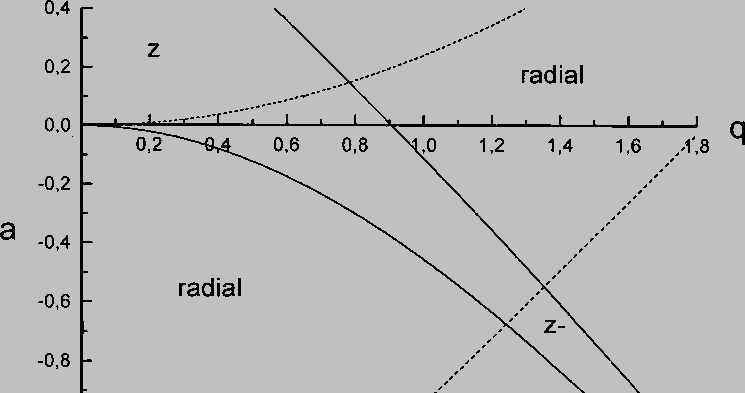
\includegraphics[scale = 0.5]{C:/Users/Baal/Desktop/Tommy/Paulstabdia.png}
	\centering
	\caption{Stabilitätsdiagramm einer Paulfalle}
	\label{stab}
\end{figure}



\subsection{Mie-Streuung}

Mie-Streuung bezeichnet Streuung von Licht an  sphärischen, homogenen Partikeln. Im Grenzfall großer Radien bekommt man die Gesetze der geometrischen Optik, für kleine Radien die Rayleight-Streuung. Die Mie-Streuung ist beschränkt auf Teilchen mit dem Durchmesser von der Größenordnung der Wellenlänge des verwendeten Lichtes.
Größenparameter ist hierbei k= $\frac {2\pi r}{\lambda}$, ist dieser in der Größenordnung von 1 bilden sich ein Beugungsmuster aus, deren Maxima und Minima vom Größenparameter abhängt.
Die theoretischen Probleme der Lichtstreuung an solch einem Partikel besteht im wesentlichen aus der Lösung der Maxwell-Gleichung mit Stetigkeitsbedingungen an dessen Oberfläche. Ein Ergebniss ist das die Intensitätsverteilung sowie Minima und Maxima rückschlüsse auf den Brechungsindex des Partikels und dessen Abmessungen geben.

\subsection{Verdampfungsprozess}

Die Verdampfung von Teilchen bei T = konst. beschreibt die Teilchendiffusion. Folgende Differenzialgleichung lässt sich für den Radius des Teilchen aufstellen:\\

$\frac{dr}{dt}= -\frac {S}{2r} \leftrightarrow \frac {d}{dt}r^2(t)=-S
$

Der Verdampfungsparameter S ist hierbei von der Umgebungstemeratur und dem Druck abhängig. Nun Integriert man die Differetialgleichung und so erhält man eine Gleichung für die Oberfläche des Teilchen in Abhängigkeit von $r_0$ Radius zum Zeitpunkt $t_0$. 

\begin{equation}
r^2(t)= r_0^2-S(t-t_0)
\label {6}
\end{equation}





\subsection{Bestimmung der Massenlandungsdichte Q/m}

Ein geladenes Teilchen das sich in Ruhe in einem elektrischen Feld befindet, hierbei kompensiert die Gewichtskraft genau die Coulomb-Kraft.\\


$F_{Gewicht}=F_{Coulomb}$
	\\
Die Gewichtskraft ist $F_{Gewicht}=mg$. Die Coulomb-Kraft eines homogenen elektrischen Feldes muss mit Hilfe eines Korrekturfaktors genähert werden (K=0.798). \\

$F_{Coulomb}=Q\frac{U}{2z_0}K=Q\frac{U}{\sqrt2 r_0}0.798$

Jetzt setzt man nun beide Kräfte gleich und dann folgt für Q/m mit $r_0 $ und g = 9.81 $\frac{m}{s^2}$:

\begin{equation}
\frac{Q}{m}=\frac{\sqrt2 r_0 g}{0.798 U}
\label {7}
\end{equation}

\section{Versuchsaufbau}

Der Versuchsaufbau besteht aus einer Paulfalle, einem Helium-Neon-Laser und einer digitalen Videokamera. Der Laserstrahl wird auf das Zentrum der Paulfalle gerichtet und das Streulicht mit der Kamera aufgenommen. Die Streulichtintensität wird dann mit einem Computerprogramm analysiert.

\begin{figure}[h]
	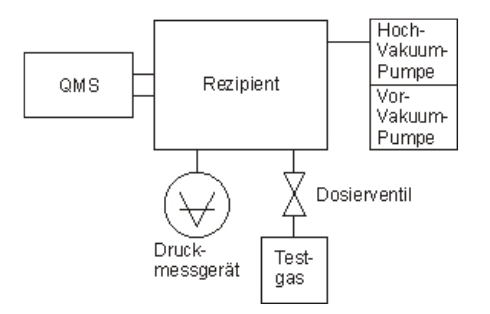
\includegraphics[scale = 0.5]{C:/Users/Baal/Desktop/Tommy/aufbau.png}
	\centering
	\caption{ Skizze des Versuchsaufbaus, mit den Komponenten (1) Paulfalle, (3) PiezoInjektor, (5) Linsensystem, (6) CCD-Kamera und (7) Messcomputer}
	\label{aufbau}
\end{figure}

\section{Durchführung}


Als erstes nahmen wir eine Eichkurve \ref{eichkurve} der Spannungsquelle auf, da die Analoganzeigen falsch waren. Zunächst wurde die Falle mit einer angelegten Wechselspannungsamplitude von 250 V mit
einer Frequenz von 100 Hz in Betrieb genommen. Dann wurden die Glaskügelchen mittels
eines Glasstäbchens in die Paulfalle gebracht. Das Bild der Kamera zeigte den mit
einem HeNe-Laser beleuchteten Probenbereich der Falle und die Kügelchen, die durch die
Falle fielen. Um die Kügelchen zu fangen, wurde die Gleichspannung zwischen Deckel und
Bodenelektrode variiert.
Nach ein paar Versuchen konnten mehrere Glaskugeln in der Falle gefangen werden.
Bei Erhöhung der Gleichspannung U wurde das Teilchen nach oben verschoben. Diese Glaskügelchen haben wir mit dem Programm view mie scattering.vi auf dem PC angesehen und Spannungen aufgenommen als diese in schwebe waren. Wir konnten von 3 Glaskügelchen den Q/m Wert bestimmen. Als nächstes entfernten wir die Glaskügelchen aus der Falle und erzeugten mit einer piezoelektrisch betriebene Düse Aerosoltröpchen um die Verdampfungskonstante zu bestimmen. Davor brauchten wir jedoch den Mittelpunkt der Aufnahme sowie Breite. Die Beleuchtung der levitierten Teilchen erfolgt durch einen HeNe-Laser. Die Verdampfungskonstante haben wir an 3 Teilchen bestimmt und diese eine Zeit lang beobachtet bis das Teilchen weg war.

\end{document}